\documentclass[../analysisII_notes.tex]{subfiles}
\begin{document}
\section{Aula 22 - 09 de Junho, 2025}
\subsection{Motivações}
\begin{itemize}
	\item Diferenciabilidade de Aplicações de Várias Variáveis Reais.
\end{itemize}
\subsection{Diferenciabilidade de Aplicações de Várias Variáveis Reais.}
Quando tratamos de casos em maiores dimensões, para podermos falar de funções, números, propriedades e etc, precisamos introduzir um sistema de coordenadas -- uma associação númerica, para cada ponto de uma \textit{superfície}, capaz de traduzir a localização do objeto estudado. Por exemplo, um ponto v em três dimensões requer a associação de 3 números para representá-lo:
\[
	v = (x, y, z),\quad x,y,z\in \mathbb{R}.
\]
Isto por si só já se mostra bem útil, tanto para descrever fenômenos reais, quanto modelagens de outras coisas. A própria física já faz uso disso direto e reto. Mas para que estudar a diferenciabilidade de aplicações que levam pontos multidimensionais em outros pontos multidimensionais?

Levando a física em conta ainda, quando formulamos uma Lei Física, muitas vezes temos apenas a taxa com que uma grandeza varia em relação a outra. Se não temos somente isso, é esta relação que descreve dado fenômeno, tal como a segunda Lei de Newton, que relaciona a força impressa sobre um corpo como um valor dependendo da variação da velocidade em relação ao tempo:
\[
	F = m a = m \frac{\mathrm{d}v}{\mathrm{d}t} = m \frac{\mathrm{d}^{2}x}{\mathrm{d}t^{2}}.
\]
De cara, já vemos que, para ela poder ser utilizada em corpos que se movem no espaço tridimensional, precisaremos generalizar as teorias e ideias de derivação vistas para o caso unidimenisonal.

Sem mais delongas, vamos às considerações inicias da formalização.
\begin{def*}
	Dados E e F espaço vetoriais sobre \(\mathbb{R}\), u e v elementos de E e \(\lambda \) um escalar, indica-se por
	\[
		\mathcal{L}(E; F)\coloneqq \{T:E\rightarrow F:\; T(u+\lambda v) = Tu + \lambda Tv\}.
	\]
	Quando \(E = F\), denotaremos apenas por \(\mathcal{L}(E)\); além disso, se \(F=\mathbb{R}\), o espaço
	\[
		E^{*}\coloneqq \mathcal{L}(E; \mathbb{R})
	\]
	será chamado \textbf{espaço dual de E}, e um elemento \(T\) em \(E^*\) será chamado \textbf{funcional (ou forma) linear em E}. \(\square\)
\end{def*}
\begin{def*}
	Se E e F são espaços normados e a dimensão de E é finita, então dado T em \(\mathcal{L}(E; F)\), definimos sua \textbf{norma} por
	\[
		\Vert T \Vert_{\mathcal{L}(E; F)} = \Vert T \Vert \coloneqq \sup_{\Vert u \Vert_{E}=1}\Vert Tu \Vert_{F}. \quad \square
	\]
\end{def*}
\begin{def*}
	Se r for um número natural maior ou igual a 2, uma função
	\[
		\varphi :E^{r}\coloneqq \underbrace{E \times E \times \dotsc \times E}_{\text{r-vezes}}\rightarrow F
	\]
	é dita \textbf{r-linear} quando, fixados \(i = 1, 2, \dotsc , r\) qualquer e \(u_{1}, \dotsc , u_{i-1}, u_{i+1}, \dotsc , u_{v}\) em E,
	\[
		\varphi (u_1, \dotsc , u_{i-1}, \underbrace{u + \lambda v}_{\mathclap{\text{i-ésima}}}, u_{i+1}, \dotsc , u_{r}) = \varphi (u_{1}, \dotsc , u, \dotsc , u_{r}) + \lambda \varphi (u_{1}, \dotsc , v, \dotsc ,u_{r})
	\]
	para todos u, v em E e \(\lambda \) real. Denotamos o espaço das funções r-lineares por
	\[
		\mathcal{L}_{r}(E; F)\coloneqq \{\varphi :E^{r}\rightarrow F:\; \varphi \text{ é r-linear}\}.
	\]
	Em particular, se \(F = \mathbb{R}\), então
	\[
		\mathcal{L}_{r}(E; \mathbb{R}) = \mathcal{L}_{r}(E)
	\]
	e seus elementos são chamados \textbf{formas r-lineares}. \(\square\)
\end{def*}
\begin{tcolorbox}[
		skin=enhanced,
		title=Observação,
		fonttitle=\bfseries,
		colframe=black,
		colbacktitle=cyan!75!white,
		colback=cyan!15,
		colbacklower=black,
		coltitle=black,
		drop fuzzy shadow,
		%drop large lifted shadow
	]
	Um caso específico importante de formas r-lineares é o de
	\[
		\mathfrak{A}_{r}(E) = \{\varphi \in \mathcal{L}_{r}(E):\;u_{i}= u_{j},\; i\neq j \Rightarrow \varphi(u_1, \dotsc , u_r) = 0\},
	\]
	cujos elementos são as chamadas \textbf{r-formas lineares alternadas}: as formas r-lineares que se anulam quando houver elementos iguais em posições diferentes.
\end{tcolorbox}
No caso da norma, se E for de dimensão finita e E e F forem espaços normados, então a norma de \(\varphi \) em \(\mathcal{L}_{r}(E; F)\) é dada por
\[
	\Vert \varphi  \Vert_{\mathcal{L}_{r}(E; F)} = \Vert \varphi  \Vert = \sup_{\Vert u_{i} \Vert_{E} = 1}\Vert \varphi(u_1, \dotsc , u_r) \Vert_{F}.
\]
Em particular, dados \(u_1, \dotsc , u_r\) em E, vale que
\[
	\Vert \varphi (u_1, \dotsc , u_{r}) \Vert_{F} \leq c \Vert u_{1} \Vert_{E}\dotsc \Vert u_{r} \Vert_{E},
\]
que tem um caso especial muito interessante quando todas as entradas são as mesmas:
\[
	\Vert \varphi (u, \dotsc , u) \Vert_{F}\leq c\Vert u \Vert^{r}.
\]
\begin{example}
	O primeiro exemplo é altamente importante -- o \textbf{produto interno euclideano}, dado por
	\begin{align*}
		\left< \cdot , \cdot  \right>: & \mathbb{R}^{n}\times \mathbb{R}^{n}\rightarrow  \mathbb{R}                           \\
		                               & (x, y)\longmapsto \left< x, y \right> = x \cdot y = \sum\limits_{i=1}^{n}x_{i}y_{i}, \\
		                               & x = (x_1, \dotsc , x_{n}) \quad\&\quad y = (y_1,\dotsc ,y_{n}).
	\end{align*}
	Neste caso, \(\left< \cdot , \cdot  \right>\in \mathcal{L}_{2}(\mathbb{R}^{n})\). Nas nossas notações, r vale 2, \(E = \mathbb{R}^{n}\) e F é \(\mathbb{R}\).
\end{example}
\begin{example}
	Outro exemplo comum é o \textbf{produto vetorial}
	\begin{align*}
		\times : & \mathbb{R}^{3}\times \mathbb{R}^{3}\rightarrow \mathbb{R}^{3} \\
		         & (u, v)\mapsto u \times v,
	\end{align*}
	em que o elemento \(u\times v\) satisfaz
	\begin{itemize}
		\item[i)] \(u\times v\) é ortogonal ao u e ao v:
		      \[
			      u\times v \perp u \quad\&\quad u\times v\perp v;
		      \]
		\item[ii)] A norma de \(u\times v\), \(\Vert u\times v \Vert_{\mathbb{R}^{n}},\) é exatamente a área do paralelogramo de lados u e v
		\item[iii)] A base \(\mathcal{B} = (u, v, u\times v)\) é uma base positiva  de \(\mathbb{R}^{3}\), isto é,
		      \[
			      \det{(u, v, u\times v)} > 0.
		      \]
		      Noutras palavras, ele satisfaz a regra da mão-direita.
	\end{itemize}
\end{example}
\begin{example}[Top 2 Conceitos Matemáticos pro Édinho]
	O determinante de uma matriz quadrada \(X\in \mathbb{M}_{n}(\mathbb{R})\) é interpretado como uma função das n colunas de X, de moto que
	\begin{align*}
		\det: & \overbrace{\mathbb{R}^{n}\times \mathbb{R}^{n}\times \dotsc \times \mathbb{R}^{n}}^{\text{n-vezes}}= \mathbb{R}^{n\times n}\rightarrow \mathbb{R} \\
		      & X \mapsto \det{(X)} = \det{\begin{bmatrix}
				                                   a_{11} & a_{12}  & \dotsc & a_{1n} \\
				                                   a_{21} & a_{22}  & \dotsc & a_{2n} \\
				                                   \vdots & \vdots  & \ddots & \vdots \\
				                                   a_{n1} & a_{n-2} & \dotsc & a_{nn}
			                                   \end{bmatrix}} = \det{[u_{1}, u_{2}, \dotsc , u_{n}]},
	\end{align*}
	em que
	\[
		u_{j} = (a_{1j}, a_{2j}, \dotsc , a_{nj})^{T}.
	\]
	Sabemos que o determinante é n-linear em \(\mathbb{R}\) e, mais ainda, que ele zera se duas colunas são iguais -- em outras palavras,
	\[
		\det\in \mathfrak{A}_{n}(\mathbb{R}^{n}).
	\]
\end{example}
\begin{def*}
	Seja \(f:U \subseteq_{ab}\mathbb{R}^{m} \rightarrow \mathbb{R}^{n}\), sendo m e n número naturais finitos. Dizemos que \textbf{f é derivável no ponto a} de seu domínio quando existe uma transformação T em \(\mathcal{L}(\mathbb{R}^{m}, \mathbb{R}^{n})\) de modo que \(r:U_{a}\rightarrow \mathbb{R}^{n}\), onde
	\[
		U_{a}\coloneqq U-a = \{h\in \mathbb{R}^{m}: a + h \in U\},
	\]
	é definido como
	\[
		r(h)\coloneqq f(a+h) - f(a) - Th
	\]
	e cumpre
	\[
		\lim_{h\to 0}\frac{r(h)}{|h|} = 0. \quad \square
	\]
\end{def*}
Como de costume, se a definição acima vale para todos os pontos de U, diremos apenas que f é derivável.
\begin{figure}[H]
	\begin{center}
		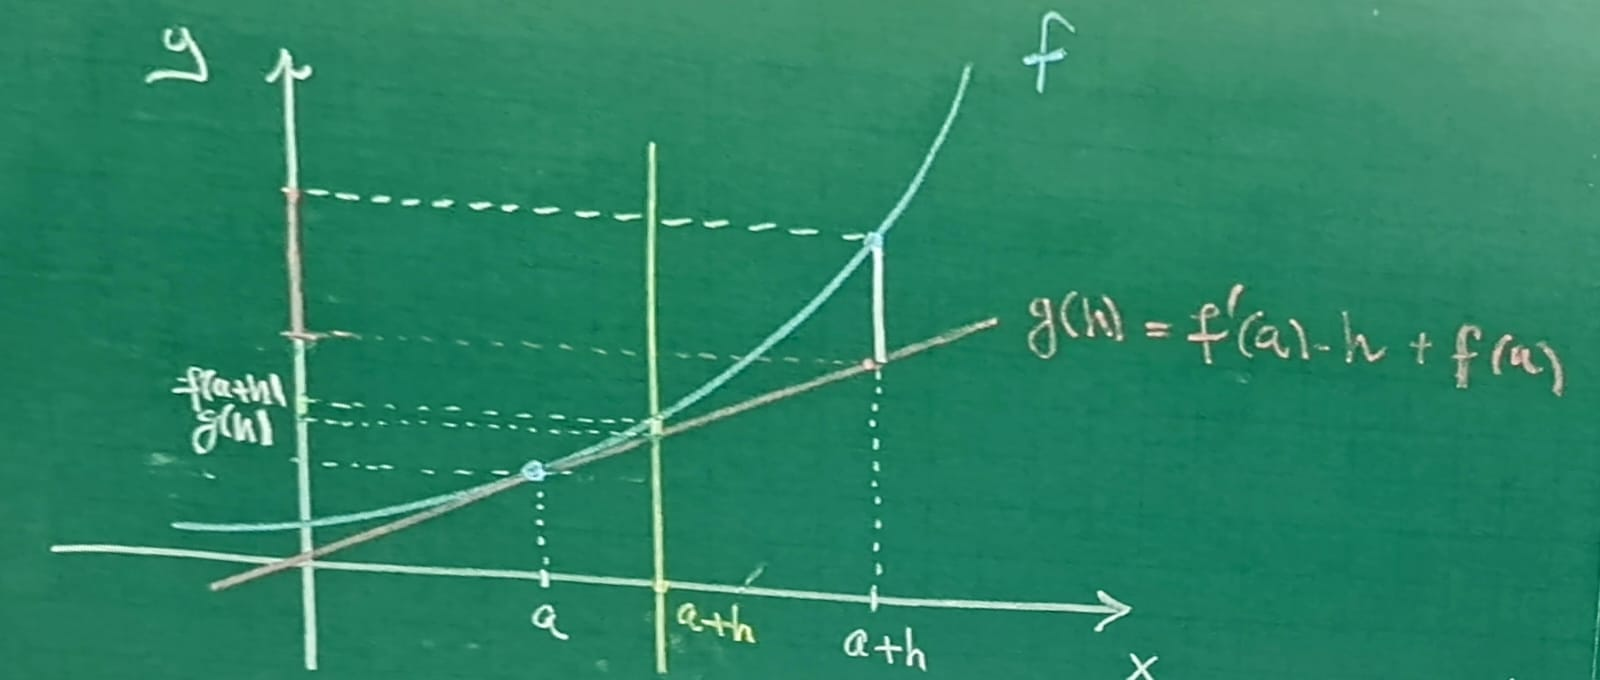
\includegraphics[height=0.5\textheight, width=0.5\textwidth, keepaspectratio]{./Images/derivative_22.png}
	\end{center}
	\caption{aqui, segue que \(f(a+h)-g(h) = f(a+h)-f'(a)h - f(a) = r(h)\).}
	\label{der22}
\end{figure}
Nesse sentido, a derivada é a melhor aproximação da f de uma função linear.
\begin{theorem*}
	Se f é derivável em a, então a T satisfazendo a definição da derivada é única.
\end{theorem*}
\begin{proof*}
	Com efeito, suponha que existam T e S transformações lineaers de \(\mathbb{R}^{m}\) em \(\mathbb{R}^{n}\) que cumprem a condição da definição. Então,
	\begin{align*}
		 & r(h) = f(a+h) - f(a) - Th \Rightarrow \lim_{h\to 0}\frac{r(h)}{|h|} = 0         \\
		 & \rho(h) = f(a+h) - f(a) - Sh \Rightarrow \lim_{h\to 0}\frac{\rho (h)}{|h|} = 0.
	\end{align*}
	Feito isso, se \(t\neq 0\) e \(h\in \mathbb{R}^{m}\) é não-nulo também, então
	\[
		Th = \frac{1}{t}T(th) = \frac{1}{t}[f(a+th) - f(a) - r(th)]
	\]
	e
	\[
		Sh + \rho (h) = f(a+h) - f(a).
	\]
	Consequentemente,
	\[
		Th = \frac{1}{t}[f(a+th) - f(a) - r(th)] = \frac{1}{t}[S(th) + \rho (th) - r(th)] = S(h) + \frac{\rho (th)}{t}-\frac{r(th)}{t}.
	\]
	Dividindo pela norma de h e passando o limite, temos para todo h diferente de 0
	\[
		Th = Sh + |h|\biggl[\frac{\rho (th)}{t|h|} - \frac{r(th)}{t|h|}\biggr]\overbracket[0pt]{\longrightarrow}^{t\to 0^{+}} Th = Sh.
	\]
	Portanto, como elas são lineares, o caso de h = 0 também é uma igualdade, permitindo que concluamos
	\[
		Th = Sh,\; \forall h\in \mathbb{R}^{n} \Rightarrow T = S. \quad \text{\qedsymbol}
	\]
\end{proof*}
Como a T é única, podemos denotá-la por um símbolo sem ambiguidade. De fato,
\begin{def*}
	A \textbf{derivada de f em a} é indicada por
	\[
		f'(a) = T\in L(\mathbb{R}^{m}, \mathbb{R}^{n}),
	\]
	em que T é a única transformada que satisfaz a definição. \(\square\)
\end{def*}
\end{document}
